\documentclass[a4paper, 12pt]{article}
\usepackage[utf8]{inputenc}
\usepackage[brazil]{babel}
\usepackage{amstext} 	% need for \text command
\usepackage{amsmath}    % need for subequations
\usepackage{graphicx}   % need for figures
\usepackage{verbatim}   % useful for program listings
\usepackage{color}      % use if color is used in text
\usepackage{subfigure}  % use for side-by-side figures
\usepackage{hyperref}   % use for hypertext links, including those to external documents and URLs
\usepackage{pictexwd}	% use for pictex graphs

%\author{Vítor M. Martins}
\title{PME2352}

\begin{document}
\maketitle
%\newpage
%\tableofcontents
%\newpage

\section{Ex 1}
%\subsection{•}
%\paragraph{•}

\begin{figure}[h]
\begin{center}
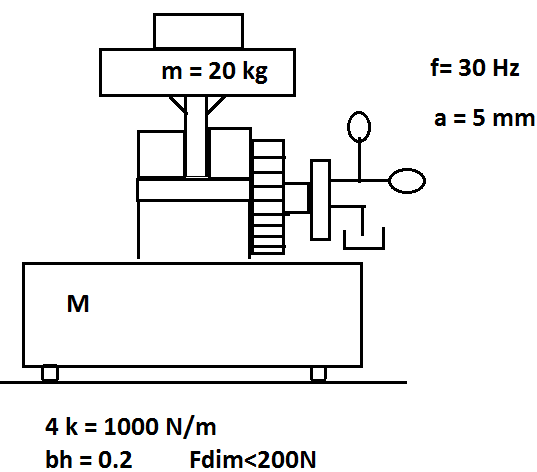
\includegraphics[scale=0.48]{./fig/1.png}
\caption{\label{fig:tur}figura Ex 1} 
\end{center}
\end{figure}
  
\[(M+m)\ddot{x}_{CM}=M\ddot{x}+m(\ddot{[a\sin (\omega_{f}t)+x}])=-4kx-c_{eq}\dot{x}\]
 
\[(M+m)\ddot{x}+\frac{4kb_{h}}{w_{f}}\dot{x}+4kx=ma\omega_{f}^{2}\sin(w_{f}t)\]
 
\[x_{p}(t)=X_{p}*\sin(\omega_f t-\psi)\]
 
\[X_{p}=\frac{\frac{ma\omega_{f}^{2}}{4k}}{\sqrt{(1-r^{2})^{2}+(4k)^{2}}}\]
 
\[\omega=\sqrt{\frac{4k}{M+m}}\]

\[\varsigma=\frac{4kb_{h}}{w_f2\sqrt{4k(M+m)}}\] 
 
\[r=\frac{w_{f}}{\omega}\]


\[2\varsigma r= \frac{4kb_{h}}{\omega_{f}\sqrt{4k(M+m)}}*\frac{\omega_f}{\omega\sqrt{M+m}}  \]
 
\[{\sqrt{4k}} = b_{h}\]
 
\[X_{p}=\frac{\frac{ma\omega_f ^{2}}{4k}}{\sqrt{(1-r^{2})^{2}+(b_{h}^{2})}}\]
 
\[F_{f}=4kx_{p}(t)+c_{eq}\dot{x_{p}}(t)=4kX_{p}\sin(\omega_{f}-\psi)+c_{eq}X_{p}\omega_{f}cos(\omega_{f}-\psi)
\]
 
\[=4kX_{p}*(\sin(\omega_{f}-\psi)+(\frac{c_{eq}\omega_{f}}{4k})cos(\omega_{f}-\psi))\]
 
\[=4kX_{p}\sqrt{1+b_{h}^{2}}\sin(\omega_f-\psi+\alpha)\]

\[\frac{\frac{ma\omega_f ^{2}}{4k}}{\sqrt{(1-r^{2})^{2}+(b_{h}^{2})}} <= 200N\] 

\[\frac{20*0.005*(30*2\pi)^{2}*\sqrt{1+0.04}}{\sqrt{(1-r^{2})^{2}+0.04}}<200\]
 
\[\frac{(20*0.005*(30*2*\pi)2)^{2}*(1+0.04)}{(200)^{2}}=(r^{2}-1)^{2}+0.04\]
 
\[r = 4.4 = \frac{\omega_{f}}{\omega}\]
 

\[\omega = \sqrt{\frac{10^{6}}{M+20}}\] 

Portanto, $\omega=43$ rad/s e M = 520 kg

\section{Ex 2}

\[c_{eq} = c(\frac{a}{b})^{2}\]
\[k_{eq}= k(\frac{a}{b})^{2}\]
\[\frac{c_{eq}}{c_{c}}=0.9\] 

\[\omega=\sqrt{\frac{k_{eq}}{M}} = 2.2 \pi\]

\[k_{eq}=16 \pi^{2}M\]

\[c_{eq} = 2\sqrt{M_{eq}K_{eq}}*0.9\]


\begin{figure}[h]
\begin{center}
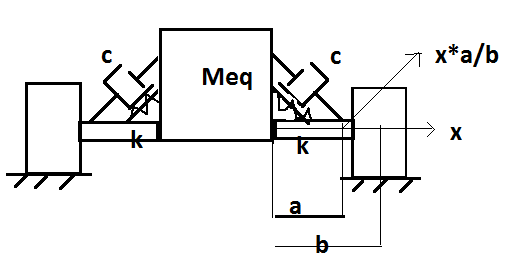
\includegraphics[scale=0.88]{./fig/2.png}
\caption{\label{fig:tur}figura 1 Ex 2} 
\end{center}
\end{figure}

\[F = Kx\frac{a}{b}\frac{\sqrt{2}}{2}\]
\[x\frac{a}{b}\frac{\sqrt{2}}{2}\]

 
\begin{figure}[h]
\begin{center}
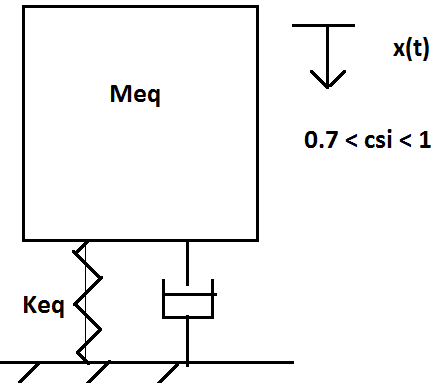
\includegraphics[scale=0.38]{./fig/3.png}
\caption{\label{fig:tur}figura 2  Ex 2} 
\end{center}
\end{figure}

\[F_{pMec}=kx(\frac{a}{b})^{2}*\frac{1}{2}\]

\begin{figure}[h]
\begin{center}
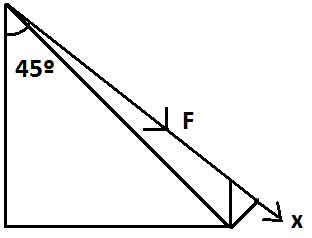
\includegraphics[scale=0.48]{./fig/4.png}
\caption{\label{fig:tur}figura 3  Ex 2} 
\end{center}
\end{figure}

\section{Ex 3}

\begin{figure}[h]
\begin{center}
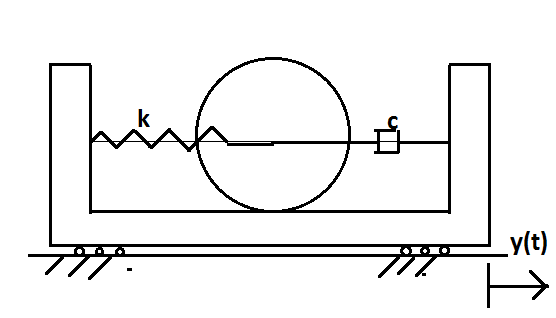
\includegraphics[scale=0.6]{./fig/5.png}
\caption{\label{fig:tur}figura 1  Ex 3} 
\end{center}
\end{figure}

\[y(t)=y_{o}\sin(\omega_{f}t)\]
\[c = \sqrt{Km}\]
TMB:\[\ \ \ \  m(\ddot{y+x}) = T - c\dot{x}-Kx \]

TMA:\[\ \ \ \  \frac{mR^{2}}{2}\ddot{\theta} = -T*R \]
\begin{figure}[h]
\begin{center}
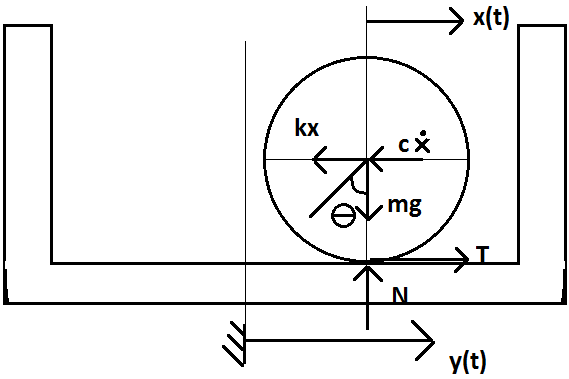
\includegraphics[scale=0.5]{./fig/6.png}
\caption{\label{fig:tur}figura 2  Ex 3} 
\end{center}
\end{figure}

Portanto: $\ \ \ \  \frac{m\ddot{x}}{2}=-T $
	\[ \theta R=x \]
	\[\theta = \frac{x}{R}\]
	\[	m(\ddot{x}+\ddot{y})+c\dot{x}+kx=\frac{-m\ddot{x}}{2}\]
	\[\frac{3}{2}m\ddot{x}+c\dot{x}+kx=-m\ddot{y}=my_{o}\omega_{f}^{2}\sin(\omega_{f}t)\]
	\[x_{p}(t)=\frac{\frac{my_{0}w_{f}^{2}}{k}}{\sqrt{(1+r^{2})^{2}+(2\zeta)^{2}}}\sin(\omega_{f}t-\psi)\]
\[	\psi=\arctan(\frac{2\zeta r}{1-r^{2}})\]
	Na ressonância, r = 1
	\[x_{p}(t)=\frac{\frac{my_{0}w_{f}^{2}}{k}}{2\zeta}\sin(\omega_{f}t-\frac{\pi}{2})\]
	Mas $\omega_{f}=\sqrt{\frac{2k}{3m}}$  
	\[	x_{p}(t)=\frac{\frac{2Y_{0}}{3}}{2\zeta}\sin(\omega_{f}t-\frac{\pi}{2})\]
\[	\zeta=\frac{c}{2\sqrt{k\frac{3}{2}m}} = \frac{\sqrt{km}}{2\sqrt{\frac{3}{2}}\sqrt{km}}=0.41\]

\[	F_{d}=\int_{CICLO}^{}{c\dot{x}\frac{dx}{dt}\text{d}t}=\frac{1}{\omega_{f}}\int_{CICLO}^{}{\dot{c}x^{2}\text{d}(\omega_{f}t)}\]

\[ = \pi\omega_{f}x_{p res}^{2}\]

\[ = \pi\sqrt{km}\sqrt{\frac{2k}{3m}}(\frac{\psi Y_{0}}{3})^{2}\]

\[Pot = \frac{E_{d CICLO}}{\Delta T _{CICLO}} = \frac{E_{d}}{\frac{2\pi}{\omega_{f}}}\]

\url{http://www-h.eng.cam.ac.uk/help/tpl/programs/Matlab/1Bdynamics.html}\footnote{Uma página interessante que mostra o que é o que nos exercicios}
	

	
	
	


\end{document}